
\documentclass{article}

\usepackage{listings}
\usepackage{amsmath,amsfonts,amsthm,amssymb,amsopn,bm}
% \usepackage{fullpage}
\usepackage[margin=.9in]{geometry}
\usepackage{graphicx}
% \usepackage{fullpage}
% \usepackage[paper=letterpaper,margin=1in,includeheadfoot,footskip=0.25in,headsep=0.25in]{geometry}
\usepackage{url}
\usepackage[usenames,dvipsnames]{color}
% \usepackage[pdfborder={0 0 1},colorlinks=true,citecolor=black,plainpages=false]{hyperref}
\usepackage{fancyhdr}
\usepackage[ruled]{algorithm2e}
\usepackage{multirow}
\newcommand{\field}[1]{\mathbb{#1}}
\newcommand{\1}{\mathbf{1}}
% \newcommand{\E}{\mathbb{E}} % real domain
\renewcommand{\P}{\mathbb{P}} % real domain
% \newcommand{\R}{\field{R}} % real domain
% \newcommand{\C}{\field{C}} % complex domain
\newcommand{\F}{\field{F}} % functional domain

\newcommand{\T}{^{\textrm T}} % transpose


\def\diag{\text{diag}}

%% operator in linear algebra, functional analysis
\newcommand{\inner}[2]{#1\cdot #2}
\newcommand{\norm}[1]{\left\|#1\right\|}
\newcommand{\twonorm}[1]{\|#1\|_2^2}
% operator in functios, maps such as M: domain1 --> domain 2
\newcommand{\Map}[1]{\mathcal{#1}}
\renewcommand{\theenumi}{\alph{enumi}} 

\newcommand{\Perp}{\perp \! \! \! \perp}

\def\E{\mathbb{E}}
\def\P{\mathbb{P}}
\def\R{\mathbb{R}}
\newcommand{\mb}[1]{\mathbf{#1}}
\newcommand{\mc}[1]{\mathcal{#1}}


\newcommand\independent{\protect\mathpalette{\protect\independenT}{\perp}}
\def\independenT#1#2{\mathrel{\rlap{$#1#2$}\mkern2mu{#1#2}}}
\newcommand{\vct}[1]{\boldsymbol{#1}} % vector
\newcommand{\mat}[1]{\boldsymbol{#1}} % matrix
\newcommand{\cst}[1]{\mathsf{#1}} % constant
\newcommand{\ProbOpr}[1]{\mathbb{#1}}
\newcommand{\grade}[1]{\small\textcolor{magenta}{\emph{[#1 points]}} \normalsize}
\date{{}}
%\graphicspath{ {./temp_img} }
\setlength\parindent{0px}

\begin{document}
\title{Homework \#1}
\author{\normalsize{CSE 546: Machine Learning}\\
\normalsize{Prof. Kevin Jamieson} \\
\normalsize{Student: Mitchell Vollger} \\
\normalsize{Due: 10/18/18  11:59 PM}}
\maketitle


\section{Gaussians}
Recall that for any vector $u \in \R^n$ we have $||u||_2^2 = u^T u = \sum_{i=1}^n u_i^2$ and $||u||_1 = \sum_{i=1}^n |u_i|$. 
For a matrix $A \in \R^{n \times n}$ we denote $|A|$ as the determinant of $A$.
A multivariate Gaussian with mean $\mu \in \R^n$ and covariance $\Sigma \in \R^{n \times n}$ has a probability density function $p(x| \mu, \Sigma) =  \frac{1}{\sqrt{(2\pi)^n |\Sigma|}} \exp( -\frac{1}{2} (x-\mu)^T \Sigma^{-1} (x-\mu) )$ which we denote as $\mathcal{N}(\mu,\Sigma)$. \\

1. \grade{4} Let 
\begin{itemize}
\item $\mu_1 = \begin{bmatrix} 1 \\ 2 \end{bmatrix}$ and $\Sigma_1 = \begin{bmatrix} 1 & 0 \\ 0 & 2 \end{bmatrix}$
\item $\mu_2 = \begin{bmatrix} -1 \\ 1 \end{bmatrix}$ and $\Sigma_2 = \begin{bmatrix} 2 & -1.8 \\ -1.8 & 2 \end{bmatrix}$
\item $\mu_3 = \begin{bmatrix} 2 \\ -2 \end{bmatrix}$ and $\Sigma_3 = \begin{bmatrix} 3 & 1 \\ 1 & 2 \end{bmatrix}$
\end{itemize}
For each $i=1,2,3$ on a separate plot:
\begin{enumerate}
  \item Draw $n=100$ points $X_{i,1},\dots,X_{i,n} \sim \mathcal{N}(\mu_i, \Sigma_i)$ and plot the points as a scatter plot with each point as a triangle marker (Hint: use \texttt{numpy.random.randn} to generate a mean-zero independent Gaussian vector, then use the properties of Gaussians to generate $X$).
  \item Compute the sample mean and covariance matrices $\widehat{\mu}_i = \frac{1}{n} \sum_{j=1}^n X_{i,j}$ and $\widehat{\Sigma}_i = \frac{1}{n-1} \sum_{j=1}^n (X_{i,j} - \widehat{\mu}_i)^2$. 
  Compute the eigenvectors of $\widehat{\Sigma}_i$. Plot the eigenvectors as line segments originating from $\widehat{\mu}_i$ and have magnitude equal to the square root of their corresponding eigenvalues.
  \item If $(u_{i,1},\lambda_{i,1})$ and $(u_{i,2},\lambda_{i,2})$ are the eigenvector-eigenvalue pairs of the sample covariance matrix with $\lambda_{i,1} \geq \lambda_{i,2}$ and $||u_{i,1}||_2 = ||u_{i,2}||_2 = 1$, for $j=1,\dots,n$ let $\widetilde{X}_{i,j} = \begin{bmatrix} \frac{1}{\sqrt{\lambda_{i,1}}} u_{i,1}^T (X_{i,j} - \widehat{\mu}_i) \\ \frac{1}{\sqrt{\lambda_{i,2}}} u_{i,2}^T (X_{i,j} - \widehat{\mu}_i)  \end{bmatrix}$. Plot these new points as a scatter plot with each point as a circle marker. 
\end{enumerate}
For each plot, make sure the limits of the plot are square around the origin (e.g., $[-c,c] \times [-c,c]$ for some $c > 0$).


\subsection{ Q1 Answer}
The three plots can be found below. And below that, the code used to generate the plots. For some reason the ticks are not symmetric on the third plot, but if you check the code it is clear that each axis has the same limits. 
\begin{center}
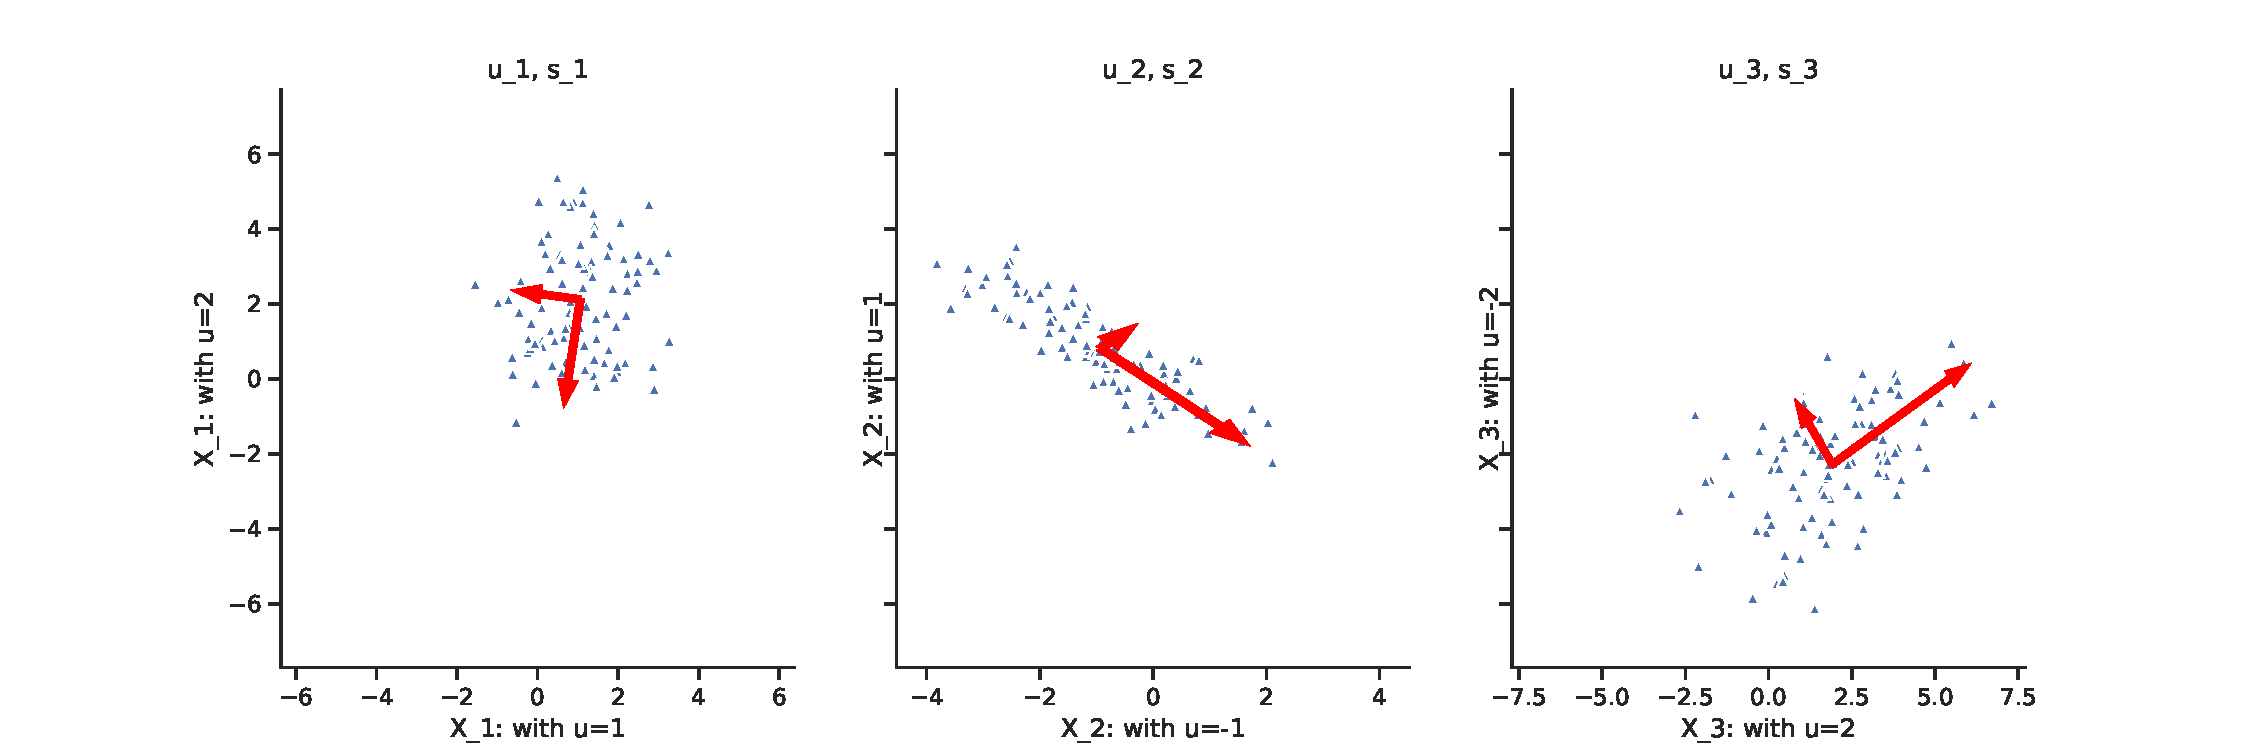
\includegraphics[width=\textwidth]{P1.pdf}
\end{center}
\lstinputlisting[language=python]{p1.py}






\section{MLE and Bias Variance Tradeoff}
Recall that for any vector $u \in \R^n$ we have $\|u\|_2^2 = u^T u = \sum_{i=1}^n u_i^2$ and $||u||_1 = \sum_{i=1}^n |u_i|$. 
Unless otherwise specified, if $P$ is a probability distribution and $x_1,\dots,x_n \sim P$ then it can be assumed each each $x_i$ is drawn iid from $P$. 
% For a matrix $A \in \R^{n \times n}$ we denote $|A|$ as the determinant of $A$.
% A multivariate Gaussian with mean $\mu \in \R^n$ and covariance $\Sigma \in \R^{n \times n}$ has a probability density function $p(x| \mu, \Sigma) =  \frac{1}{\sqrt{(2\pi)^n |\Sigma|}} \exp( -\frac{1}{2} (x-\mu)^T \Sigma^{-1} (x-\mu) )$ which we denote as $\mathcal{N}(\mu,\Sigma)$. \\

2. \grade{1}  Let $x_1,\dots,x_n \sim \text{uniform}(0,\theta)$ for some $\theta$. What is the Maximum likelihood estimate for $\theta$?\\





\subsection{Q2 Answer}

\begin{align}
    f(x) & = \frac{1}{\theta} \text{, for } 0 \le x \le \theta \\
    \implies L(\theta) & = \prod_{i=1}^n \frac{1}{\theta} \\
    & = \theta^{-n} \\
    \implies \frac{d}{d\theta} log(L) & = \frac{d}{d\theta} -n log(\theta) \\
    & = -\frac{n}{\theta} \\
\end{align}
$log(L(\theta))$ and therefore also $L(\theta)$ are decreasing functions thus the functions is minimized when $\theta$ is as large as possible. Thus the MLE for $\theta$ is:
$$\widehat{\theta} = \text{argmax}_x x_1,...,x_n $$ \\



3. \grade{2} Let $(x_1,y_1),\dots,(x_n,y_n)$ be drawn at random from some population where each $x_i \in \R^d$, $y_i \in \R$, and let $\widehat{w} = \arg\min_w \sum_{i=1}^n (y_i - w^T x_i)^2$.
Suppose we have some test data $(\widetilde{x}_1,\widetilde{y}_1),\dots,(\widetilde{x}_m,\widetilde{y}_m)$ drawn at random from the population as the training data. 
If $R_{tr}(w) = \frac{1}{n} \sum_{i=1}^n (y_i - w^T x_i)^2$ and $R_{te}(w) = \frac{1}{m} \sum_{i=1}^m (\widetilde{y}_i - w^T \widetilde{x}_i)^2$. Prove that 
\begin{align*}
\E[ R_{tr}(\widehat{w}) ] \leq \E[ R_{te}(\widehat{w}) ]
\end{align*}
where the expectations are over all that is random in each expression. Do not assume any model for $y_i$ given $x_i$ (e.g., linear plus Gaussian noise). [This is exercise 2.9 from HTF, originally from Andrew Ng.]\\


\subsection{Q3 Answer}

\begin{align}
    E[R_{tr}(\hat{w})] & = E[1/n \sum_{i=1}^n (y_i - \hat{w}^T x_i)^2] \\
    & \text{ All draws are iid so the expectation of the average of draws is the same} \\
    & \text{ as the expectation for one draw} \\
    & = E[ (y_i - \hat{w}^T x_i)^2 ] \\
\end{align}
A similar argument can be made for the test data. 
\begin{align}
    E[R_{te}(\hat{w})] & = E[1/m \sum_{i=1}^m (\~y_i - \hat{w}^T \~x_i)^2] \\
    & = E[ (\~y_i - \hat{w}^T \~x_i)^2 ] \\
\end{align}
Thus we need to show that:
\begin{align}
       E[ (y_i - \hat{w}^T x_i)^2 ] & \leq E[ (\~y_i - \hat{w}^T \~x_i)^2 ] \\
\end{align}
However $\hat{w}$ was chosen to minimize this exact function, $(y_i - \hat{w}^T x_i)^2$, so .







4.  \grade{8} Let random vector $X \in \R^d$ and random variable $Y \in \R$ have a joint distribution $P_{XY}(X,Y)$. 
Assume $\E[X]=0$ and define $\Sigma = \text{Cov}(X)=\E[(X-\E[X])(X-\E[X])^T]$ with eigenvalues $\alpha_1 \geq \alpha_2 \geq \dots \geq \alpha_d$ and orthonormal eigenvectors $v_1,\dots,v_d$ such that $\Sigma = \sum_{i=1}^d \alpha_i v_i v_i^T$.
For $(X,Y) \sim P_{XY}$ assume that $Y = X^T w + \epsilon$ for $\epsilon \sim \mathcal{N}(0,\sigma^2)$ such that $\E_{Y|X}[ Y | X=x] = x^T w$.
Let $\mathcal{D}=\{(x_i,y_i)\}_{i=1}^n$ where each $(x_i,y_i) \sim P_{XY}$.
For some $\lambda >0$ let 
\begin{align*}
\widehat{w} = \arg\min_w \sum_{i=1}^n (y_i - x_i^T w)^2 + \lambda \| w \|_2^2
\end{align*}
If $\mb{X}=[x_1,\dots,x_n]^T$, $\mb{y} = [y_1,\dots,y_n]^T$, $\boldsymbol{\epsilon} = [\epsilon_1,\dots,\epsilon_n]^T$ then it can be shown that 
\begin{align}\label{eq:ridge_soln}
\widehat{w} = (\mb{X}^T \mb{X} + \lambda I)^{-1} \mb{X}^T \mb{y}.
\end{align}
Note teh notational difference between a random $X$ of $(X,Y)\sim P_{XY}$ and the $n \times d$ matrix $\mb{X}$ where each row is drawn from $P_X$.
Realizing that $\mb{X}^T \mb{X} = \sum_{i=1}^n x_i x_i^T$, by the law of large numbers we have $\frac{1}{n} \mb{X}^T\mb{X} \rightarrow \Sigma$ as $n \rightarrow \infty$. 
In your analysis assume $n$ is large and make use of the approximation $\mb{X}^T \mb{X} = n \Sigma$.
Justify all answers.
\begin{enumerate}
    \item Show Equation~\eqref{eq:ridge_soln}.
    \item Show that $\widehat{w}$ of Equation~\ref{eq:ridge_soln} can also be written as 
    \begin{align*}
        \widehat{w} = w - \lambda (\mb{X}^T \mb{X}+\lambda I)^{-1} w + (\mb{X}^T \mb{X}+\lambda I)^{-1} \mb{X}^T \boldsymbol{\epsilon}
    \end{align*}
    \item For general $\widehat{f}_{\mc{D}}(x)$ and $\eta(x) = \E_{Y|X}[ Y | X=x]$, we showed in class that the bias variance decomposition is stated as 
    \begin{align*}
        \E_{XY,\mc{D}}[ (Y-\widehat{f}_{\mc{D}}(X))^2] &= \E_{X}\Big[\E_{Y|X,\mc{D}}\big[(Y-\widehat{f}_{\mc{D}}(X))^2 |X=x \big] \Big]
    \end{align*}
    where
    \begin{align*}
    \E_{Y|X,\mc{D}}\big[(Y-\widehat{f}_{\mc{D}}(X))^2 |X=x \big] = \underbrace{\E_{Y|X}[ (Y-\eta(x))^2 | X=x]}_{\text{Irreducible error}} + \underbrace{(\eta(x)-\E_{\mc{D}}[\widehat{f}_{\mc{D}}(x)])^2}_{\text{Bias-squared}} +
          \underbrace{\E_{\mc{D}}[ ( \E_{\mc{D}}[\widehat{f}_{\mc{D}}(x)] - \widehat{f}_{\mc{D}}(x))^2]}_{\text{Variance}}.
    \end{align*}
    In what follows, use our particular problem setting with $\widehat{f}_{\mc{D}}(x) = \widehat{w}^T x$. \\
    Irreducible error: What is $\E_X\Big[ \E_{Y|X}[ (Y-\eta(x))^2 | X=x] \Big]$?
    \item Bias-squared: Use the approximation $\mb{X}^T \mb{X} = n \Sigma$ to show that 
    \begin{align*}\E_{X}\big[ (\eta(X)-\E_{\mc{D}}[\widehat{f}_{\mc{D}}(X)])^2 \big] = \sum_{i=1}^d \frac{\lambda^2 (w_i^T v_i)^2 \alpha_i}{(n \alpha_i + \lambda)^2} \leq \max_{j=1,\dots,d} \frac{\lambda^2 \alpha_j \|w\|_2^2}{(n \alpha_j + \lambda)^2} 
 \end{align*}
    \item Variance: Use the approximation $\mb{X}^T \mb{X} = n \Sigma$ to show that   
    \begin{align*}
    \E_{X}\big[ \E_{\mc{D}}[ ( \E_{\mc{D}}[\widehat{f}_{\mc{D}}(X)] - \widehat{f}_{\mc{D}}(X))^2] \big] = \sum_{i=1}^d \frac{\sigma^2 \alpha_i^2 n}{(\alpha_i n + \lambda)^2} \leq \frac{d \sigma^2 \alpha_1^2 n}{(\alpha_1 n + \lambda)^2}
    \end{align*}
    \item Assume $\Sigma= \alpha_1 \, I$ for some $\alpha_1 >0$. Show that for the approximation $\mb{X}^T \mb{X} = n \Sigma$ we have
    \begin{align*}
    \E_{XY,\mc{D}}[ (Y-\widehat{f}_{\mc{D}}(X))^2] = \sigma^2 + \frac{\lambda^2 \alpha_1 \|w\|_2^2}{(\alpha_1 n+\lambda)^2} + \frac{d \sigma^2 \alpha_1^2 n}{(\alpha_1 n + \lambda)^2}
    \end{align*}
    What is the $\lambda^\star$ that minimizes this expression? 
    In a sentence each describe how varying each parameter (e.g., $\|w\|_2$, $d$, $\sigma^2$) affects the size of $\lambda^\star$ and if this makes intuitive sense.
    Plug this $\lambda^\star$ back into the expression and comment on how this result compares to the $\lambda=0$ solution. It may be helpful to use $\tfrac{1}{2}(a+b) \leq \max\{a,b\} \leq a+b$ for any $a,b>0$ to simplify the expression.  
    \item Assume that $\alpha_1 > \alpha_2 = \alpha_3 = \dots = \alpha_d$ and furthermore, that $w/\|w\|_2 = v_1$. Show that for the approximation $\mb{X}^T \mb{X} = n \Sigma$ we have
    \begin{align*}
    \E_{XY,\mc{D}}[ (Y-\widehat{f}_{\mc{D}}(X))^2] = \sigma^2 + \frac{\lambda^2 \alpha_1 \|w\|_2^2}{(\alpha_1 n+\lambda)^2} + \frac{\sigma^2 n \alpha_1^2}{(\alpha_1 n + \lambda)^2} + \frac{\sigma^2 n \alpha_2^2 (d-1)}{(\alpha_2 n + \lambda)^2}
    \end{align*}
    It can be shown that $\lambda^\star = \frac{\sigma^2 + \sigma^2(d-1)\alpha_1/\alpha_2}{\|w\|_2^2}$ approximately minimizes this expression. 
    In a sentence each describe if this makes intuitive sense, comparing to the solution of the last problem.
    \item As $\lambda$ increases, how does the bias and variance terms behave?
     
\end{enumerate}

\subsection{Q4a Answer}
Re writing the equation in matrix form:
\begin{align*}
\widehat{w} & = \text{argmin}_{w} \sum_{i=0}^{n} \| w^Tx_{i} - y_{i} \|^{2}_{2} + \lambda \|w\|_{2}^{2} \\
& = \text{argmin}_w \| X_w - Y \|_2^2 + \lambda \|w\|_2^2 \\
\end{align*}
Take the derivative:
\begin{align*}
    \nabla_{w} & = 2 X^T(X w -Y) + 2 \lambda w \\
    2 X^T(X\widehat{w} -Y) + 2 \lambda \widehat{w} & = 0 \\
    X^T(X\widehat{w} -Y) + \lambda \widehat{w} & = 0 \\
    X^TX\widehat{w} + \lambda \widehat{w} & = X^T Y \\
    (X^TX + \lambda I ) \widehat{w} & = X^T Y \\
     \widehat{w} & =(X^TX + \lambda I )^{-1} X^T Y \\
\end{align*}


\subsection{Q4b Answer}

\begin{align}
    \hat{w} & = (X^TX + \lambda I)^{-1}X^T(Xw + \epsilon) \\
            & = (X^TX + \lambda I)^{-1}X^TXw + (X^TX + \lambda I)^{-1}X^T \epsilon \\
            & = (X^TX + \lambda I)^{-1}(X^TX + \lambda I - \lambda I)w + (X^TX + \lambda I)^{-1}X^T \epsilon \\
            & = w - \lambda(X^TX + \lambda I)^{-1}w + (X^TX + \lambda I)^{-1}X^T \epsilon \\
\end{align}



\subsection{Q4c Answer}
Note we were given that:
$$\eta(x) = E_{Y|X}[Y|X=x] = x^Tw$$
Thus:
\begin{align}
    E_X[E_{Y|X}[(Y-\eta(x))^2| X = x]] & = E[(x^T w + \epsilon - \eta(x))^2] \\
    & = E[(x^T w + \epsilon -  E_{Y|X}[Y|X=x])^2 ] \\
    & = E[(x^T w + \epsilon -  x^T w)^2 ] \\
    & = E[\epsilon^2 ] \\
    & = \sigma^2 \\
\end{align}


\subsection{Q4d Answer}
Let $R=(\mat{X}^T\mat{X} + \lambda I)^{-1} =(n\Sigma + \lambda I)^{-1} $
\begin{align}
     E_X[(\eta(X) - E_D[\hat{f}_D(X)])^2] & = E_X[(\eta(X) - E_D[(\hat{w}^TX])^2] \\
    & = E_X[(X^T w -E_D[(w - \lambda R w + R X^T \epsilon)^T X])^2] \\
    &= E_X[(X^T w - E_D[w^T]X +E_D[(\lambda R w)^T X] + E_D[(RX^T\epsilon)^TX])^2] \\
    & \text{By our assumptions D does not depend on R so} \\
    &= E_X[(X^T w - w^TX + (\lambda R w)^T X + E_D[\epsilon]E_D[(RX^T)^TX])^2] \\
    & \text{The $E[\epsilon] = 0 $ because it is draw from a Gaussian around 0, thus:} \\
    &= E_X[(0 + (\lambda R w)^T X + 0  E_D[(RX^T)^TX])^2] \\
    &= E_X[ ((\lambda R w)^T X)^2] \\
    &=\lambda^2 w^Tw E_X[ ( (R^T X)^2] \\
    &=\lambda^2 w^Tw R^T R * E_X[XX^T] \\
    &=\lambda^2 w^Tw R^T R * E_X[(X-0)(X-0)^T] \\
    &=\lambda^2 w^Tw R^T R * E_X[(X-E(X))(X-E(X))^T] \\
    & \text{ This final term is just the co-variance. } \\
    &=\lambda^2 w^Tw R^T R \Sigma \\
\end{align}





\section{Programming: Ridge Regression on MNIST}
5. \grade{10} In this problem we will implement a least squares classifier for the MNIST data set. The task
is to classify handwritten images of numbers between $0$ to $9$.\\

You are \textbf{NOT} allowed to use
any of the prebuilt  classifiers in \verb|sklearn|.  Feel free to use any method from \verb|numpy|
or \verb|scipy|. Remember: if you are inverting a matrix in your code, you are probably doing something wrong (Hint: look at \verb|scipy.linalg.solve|).\\

Get the data from \url{https://pypi.python.org/pypi/python-mnist}. \\
Load the data as follows:
\begin{verbatim}
from mnist import MNIST

def load_dataset():
    mndata = MNIST('./data/')
    X_train, labels_train = map(np.array, mndata.load_training())
    X_test, labels_test = map(np.array, mndata.load_testing())
    X_train = X_train/255.0
    X_test = X_test/255.0
\end{verbatim}
You can visualize a single example by reshaping it to its original $28 \times 28$ image shape.

\begin{enumerate}
\item In this problem we will choose a linear classifier to minimize the least squares objective:

\begin{align*}\widehat{W} = \text{argmin}_{W \in \R^{d \times k}} \sum_{i=0}^{n} \| W^Tx_{i} - y_{i} \|^{2}_{2} + \lambda \|W\|_{F}^{2}
\end{align*}

We adopt the notation where we have $n$ data points in our training objective 
and each data point $x_i \in \R^d$. $k$ denotes
the number of classes which is in this case equal to 10. Note that $\|W\|_{F}$ corresponds to the Frobenius norm of $W$, i.e. $\|\text{vec}(W)\|_2^2$.

Derive a closed form for $\widehat{W}$.

\item
As as first step we need to choose the vectors $y_i \in \mathbb{R}^k$ by converting the original labels (which are in $\left\{0,\ldots,9\right\})$ to
vectors.
We will use the one-hot encoding of the labels, i.e. the original label $j \in \{0, \ldots, 9\}$ is mapped to the standard basis vector $e_j$.
To classify a point $x_i$ we will use the rule $\arg\max_{j=0,\dots,9} \widehat{W}^T x_i$.

\item
Code up a function called \verb|train| that returns $\widehat{W}$ that takes as input $X \in\R^{n \times d}$, $y \in \{0,1\}^{n \times k}$, and $\lambda > 0$.
Code up a function called \verb|predict| that takes as input $W \in \R^{d \times k}$, $X' \in\R^{m \times d}$ and returns an $m$-length vector with the $i$th entry equal to $\arg\max_{j=0,\dots,9} W^T x_i'$ where $x_i'$ is a column vector representing the $i$th example from $X'$.\\

Train $\widehat{W}$ on the MNIST training data with $\lambda = 10^{-4}$ and make label predictions on the test data. What is the training and testing classification accuracy (they should both be about $85\%$)? 

\item We just fit a classifier that was linear in the pixel intensities to the MNIST data.
For classification of digits the raw pixel values are very, very bad features: it's pretty hard to separate digits with linear functions in pixel space.
The standard solution to the this is to come up with some transform $h : \mathbb{R}^d \rightarrow \mathbb{R}^p$ of the original pixel values such that the transformed points are (more easily) linearly separable.
In this problem, you'll use the feature transform:
\[
 h(x) = \cos(G x + b).
\]
where $G \in \mathbb{R}^{p \times d}$, $b \in \mathbb{R}^p$, and the cosine function is applied elementwise. 
We'll choose $G$ to be a \emph{random} matrix, with each entry sampled i.i.d. with mean $\mu=0$ and variance $\sigma^2=0.1$, and $b$ to be a random vector sampled i.i.d. from the uniform distribution on $[0,2\pi].$
The big question is: \emph{how do we choose $p$?} Cross-validation, of course!\\

Randomly partition your training set into proportions 80/20 to use as a new training set and validation set, respectively. 
Using the \verb|train| function you wrote above, train a $\widehat{W}^{p}$ for different values of $p$ and plot the classification training error and validation error on a single plot with $p$ on the $x$-axis. 
Be careful, your computer may run out of memory and slow to a crawl if $p$ is too large ($p\leq 6000$ should fit into 4 GB of memory). 
You can use the same value of $\lambda$ as above but feel free to study the effect of using different values of $\lambda$ and $\sigma^2$ for fun.

\item Instead of reporting just the classification test error, which is an unbiased estimate of the \emph{true} error, we would like to report a \emph{confidence interval} around the test error that contains the true error.
For any $\delta \in (0,1)$, it follows from Hoeffding's inequality that if $X_i$ for all $i=1,\dots,m$ are i.i.d. random variables with $X_i \in [a,b]$ and $\E[X_i] = \mu$, then with probability at least $1-\delta$ 
\begin{align*}
\P\left( \left| \left(\frac{1}{m} \sum_{i=1}^m X_i\right) - \mu \right| \geq \sqrt{\frac{\log(2/\delta)}{2m}} \right) \leq \delta
\end{align*}
We will use the above equation to construct a confidence interval around our true classification error since the test error is just the average of indicator variables taking values in $0$ or $1$ corresponding to the $i$th test example being classified correctly or not, respectively, where an error happens with probability $\mu$, the \emph{true} classification error. 

Let $\widehat{p}$ be the value of $p$ that approximately minimizes the validation error on the plot you just made and use $\widehat{W}^{\widehat{p}}$ to compute the classification test accuracy, which we will denote as $E_{test}$. 
Use Hoeffding's inequality, above, to compute a confidence interval that contains $\E[E_{test}]$ (i.e., the \emph{true} error) with probability at least $0.95$ (i.e., $\delta=0.05$).
Report $E_{test}$ and the confidence interval. 


\end{enumerate}











\subsection{Q5a Answer}

Re writing the equation in matrix form:
\begin{align*}
\widehat{W} & = \text{argmin}_{W \in \R^{d \times k}} \sum_{i=0}^{n} \| W^Tx_{i} - y_{i} \|^{2}_{2} + \lambda \|W\|_{F}^{2} \\
& = \text{argmin}_W \| X_w - Y \|_2^2 + \lambda \|w\|_2^2 \\
\end{align*}
Take the derivative:
\begin{align*}
    \nabla_{W} & = 2 X^t(X W -Y) + 2 \lambda W \\
    2 X^t(X\widehat{W} -Y) + 2 \lambda \widehat{W} & = 0 \\
    X^T(X\widehat{W} -Y) + \lambda \widehat{W} & = 0 \\
    X^TX\widehat{W} + \lambda \widehat{W} & = X^T Y \\
    (X^TX + \lambda I ) \widehat{W} & = X^T Y \\
     \widehat{W} & =(X^TX + \lambda I )^{-1} X^T Y \\
\end{align*}


\subsection{Q5b Answer}
See code for a function called "hotones". 

\subsection{Q5c Answer}
See code for train and predict functions. \\
The train accuracy was: 85.2\% \\
The test accuracy was: 85.3\% \\

\subsection{Q5d Answer}
Below is a plot showing test accuracy in red and train accuracy in blue as a function of $p$. 
\begin{center}
    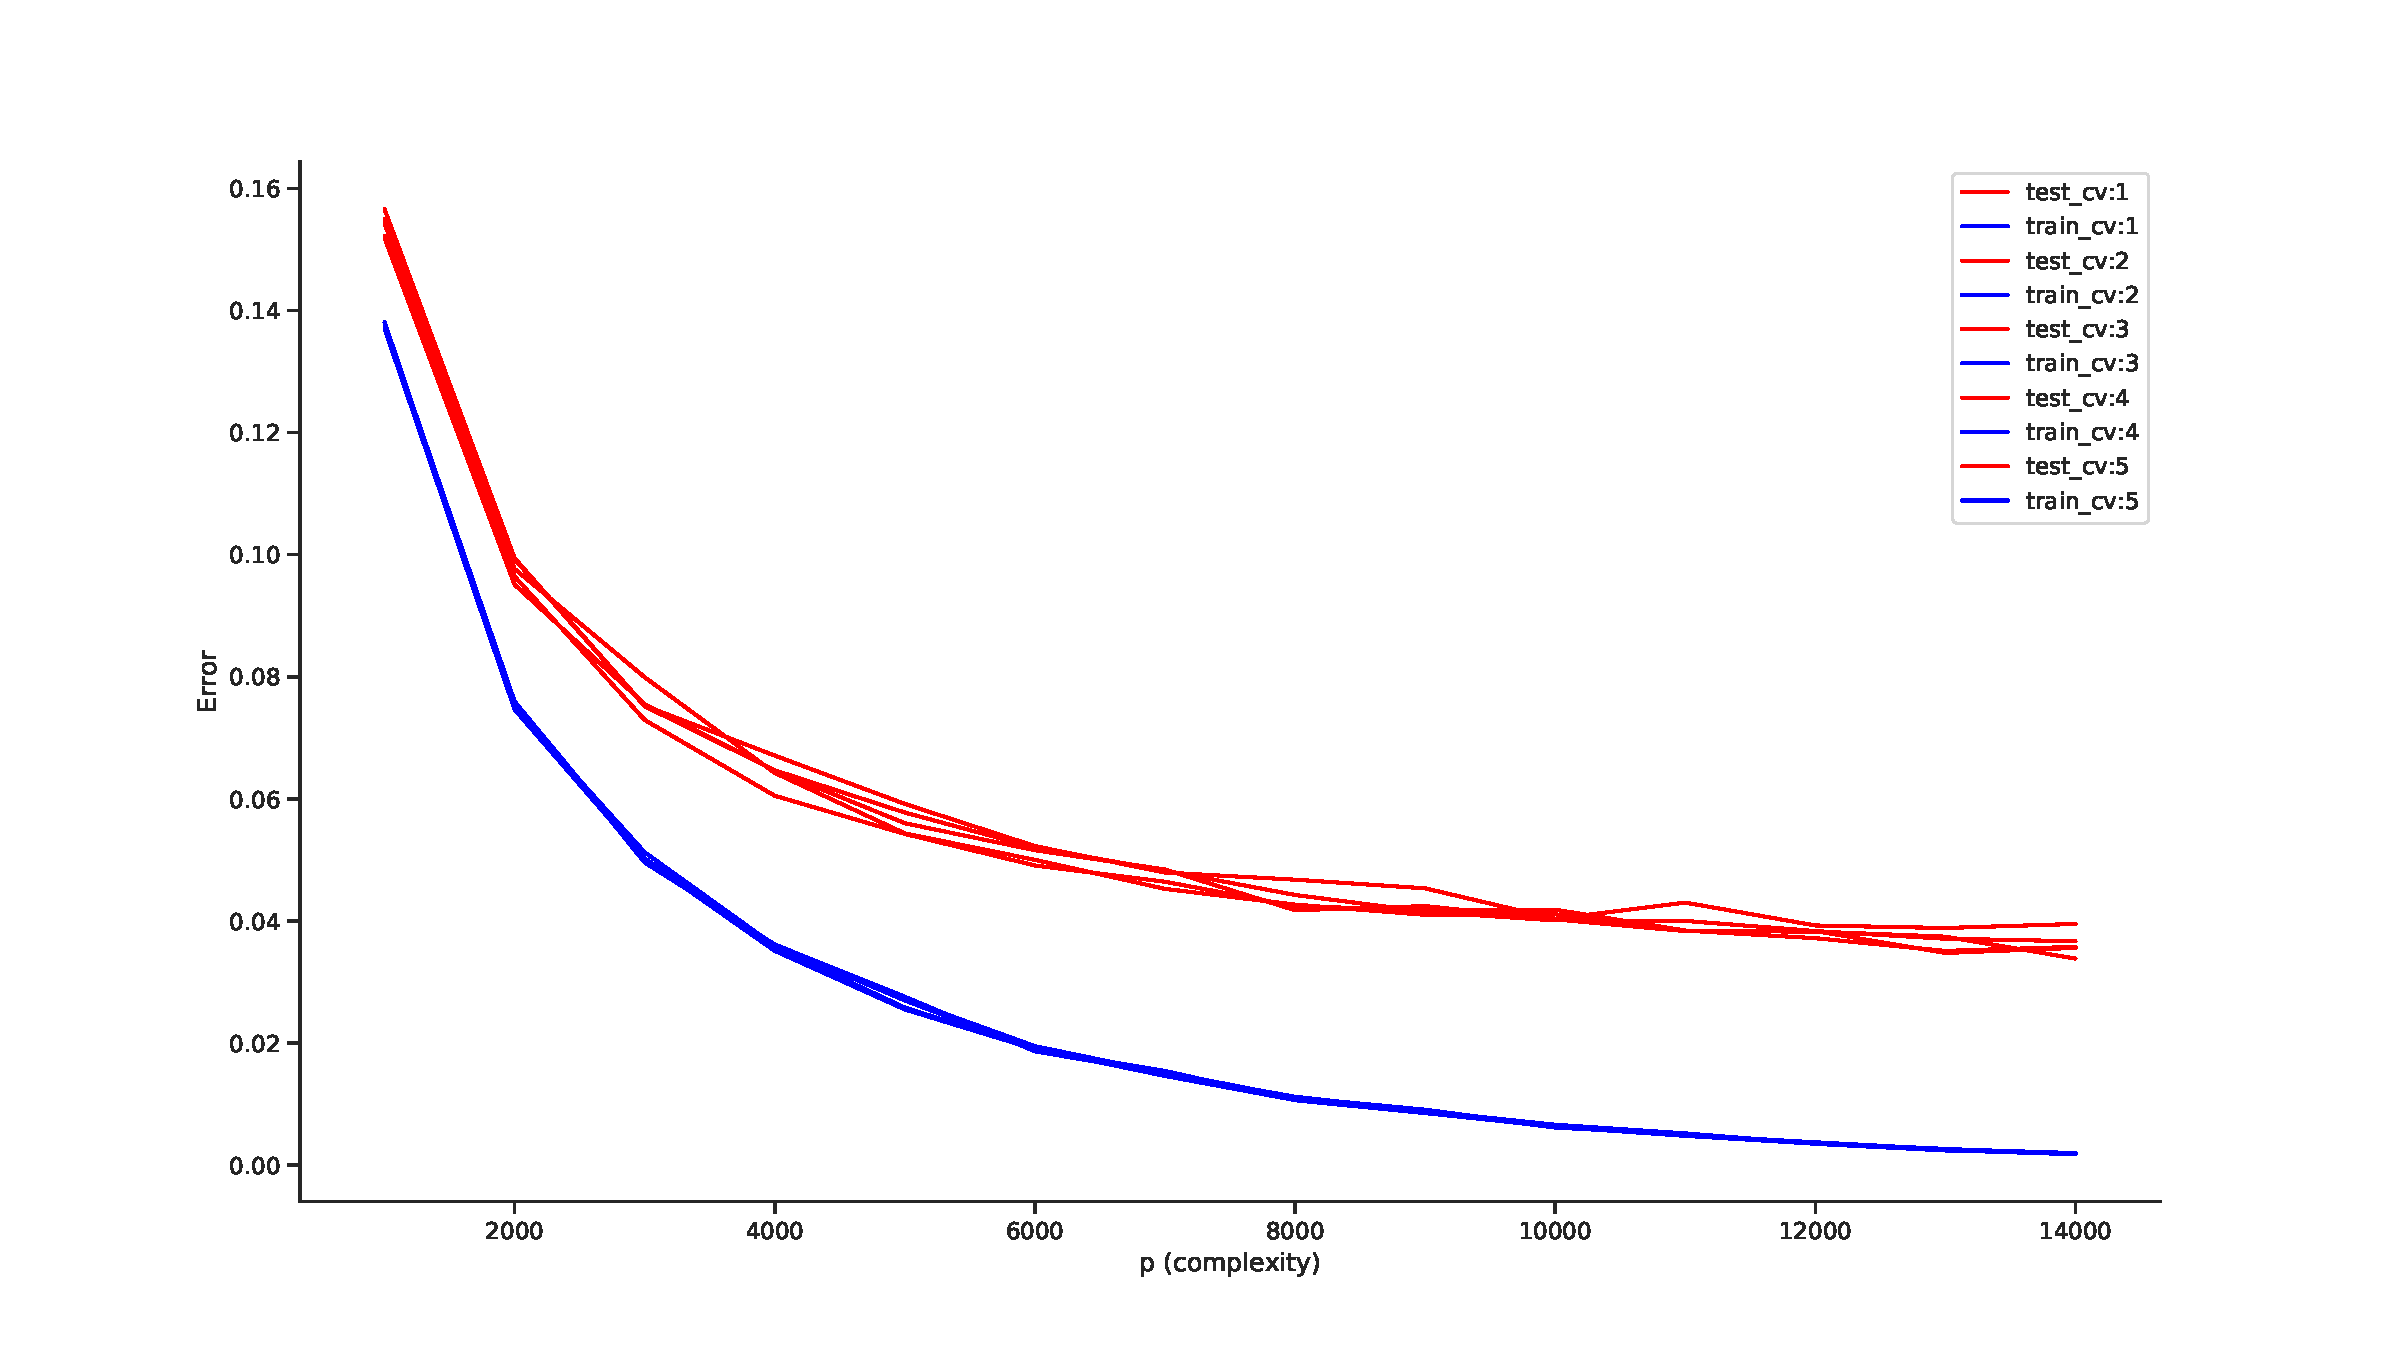
\includegraphics[width=\textwidth]{hw1/P3.pdf}
\end{center}

\subsection{Q5e Answer}

\begin{align*}
\P\left( \left| \left(\frac{1}{m} \sum_{i=1}^m X_i\right) - \mu \right| \geq \sqrt{\frac{\log(2/\delta)}{2m}} \right) & \leq \delta \\
\P\left( \left| \left(\frac{1}{m} \sum_{i=1}^m X_i\right) - \mu \right| \leq \sqrt{\frac{\log(2/\delta)}{2m}} \right) & \geq 1 - \delta \\
\P\left( \left| E_{test} - \E[E_{test}] \right| \leq \sqrt{\frac{\log(2/0.05)}{2m}} \right) & \geq 0.95 \\
\P\left( E_{test} - \sqrt{\frac{\log(2/0.05)}{2m}} \leq  \E[E_{test}]  \leq E_{test} + \sqrt{\frac{\log(2/0.05)}{2m}} \right) & \geq 0.95 \\
\end{align*}

I found that $E_{test}=0.9505$ was highest for the largest value of $p$ I could run, $p=5900$. 
The confidence interval around this value was:
$$ 0.9375 < \E[E_{test}] < 0.9635	$$
See my code for details of the calculation. 

\subsection{Q5 Code}
\lstinputlisting[language=python]{p3.py}

\end{document}
